%----------------- CHAPTER 4 -------------------------------------------
%--------NOISE-----------------------------------------------
%% Divides the noises into displacement noise and sensing noise.
%% 
%% 
%% 
\chapter{The Noises}
\label{chap:noise}

\begin{figure}[!h]
\centerline{\includegraphics[angle=0,width=6.5in]{Figures/Chap4/S3noise.pdf}}
\end{figure}
\clearpage

There are many noise sources in the LIGO interferometers. In this chapter,
those noises which contaminate the gravitational wave readout channel and are 
of a comparable amplitude to the strain noise goal are described.

The noises are categorized as either a displacement noise, one which directly
moves the suspended mirrors, or as a sensing noise, one which appears in the
readout signal but is not caused by a gravitational wave.



%- - - - - - - - - -  -  -  - - - - - - -  -  -  -   -   -    -    -     -      -
%- - -  DISPLACEMENT NOISES - - - - - - -  -  -  -   -   -    -    -     -      -
%- - - - - - - - - -  -  -  - - - - - - -  -  -  -   -   -    -    -     -      -
\section{Displacement Noises}
The displacement noises in this section are only those that cause a differential
change in the arm cavity lengths. We are also mainly concerned with noise in
the 40-7000 Hz band where the interferometer is designed to be sensitive to
gravity waves.


%-------------------------------------------------------
\subsection{Seismic Noise}
The test mass mirrors are on the earth and so vibrations of the earth's
surface could directly show up as a strain noise. A rough estimate for 
the displacement spectral density of the ground noise above 0.1 Hz at a quiet site is 
$x(f) = \frac{10^{-8}}{f^{2}} \frac{\mbox{m}}{\sqrt{\mbox{Hz}}}$. 
At 100 Hz, this would still be 7 orders of magnitude above the 
LIGO displacement noise goal. A combination of passive and active 
isolation techniques are used to reduce the seismic coupling.

\begin{figure}[!h]
\centerline{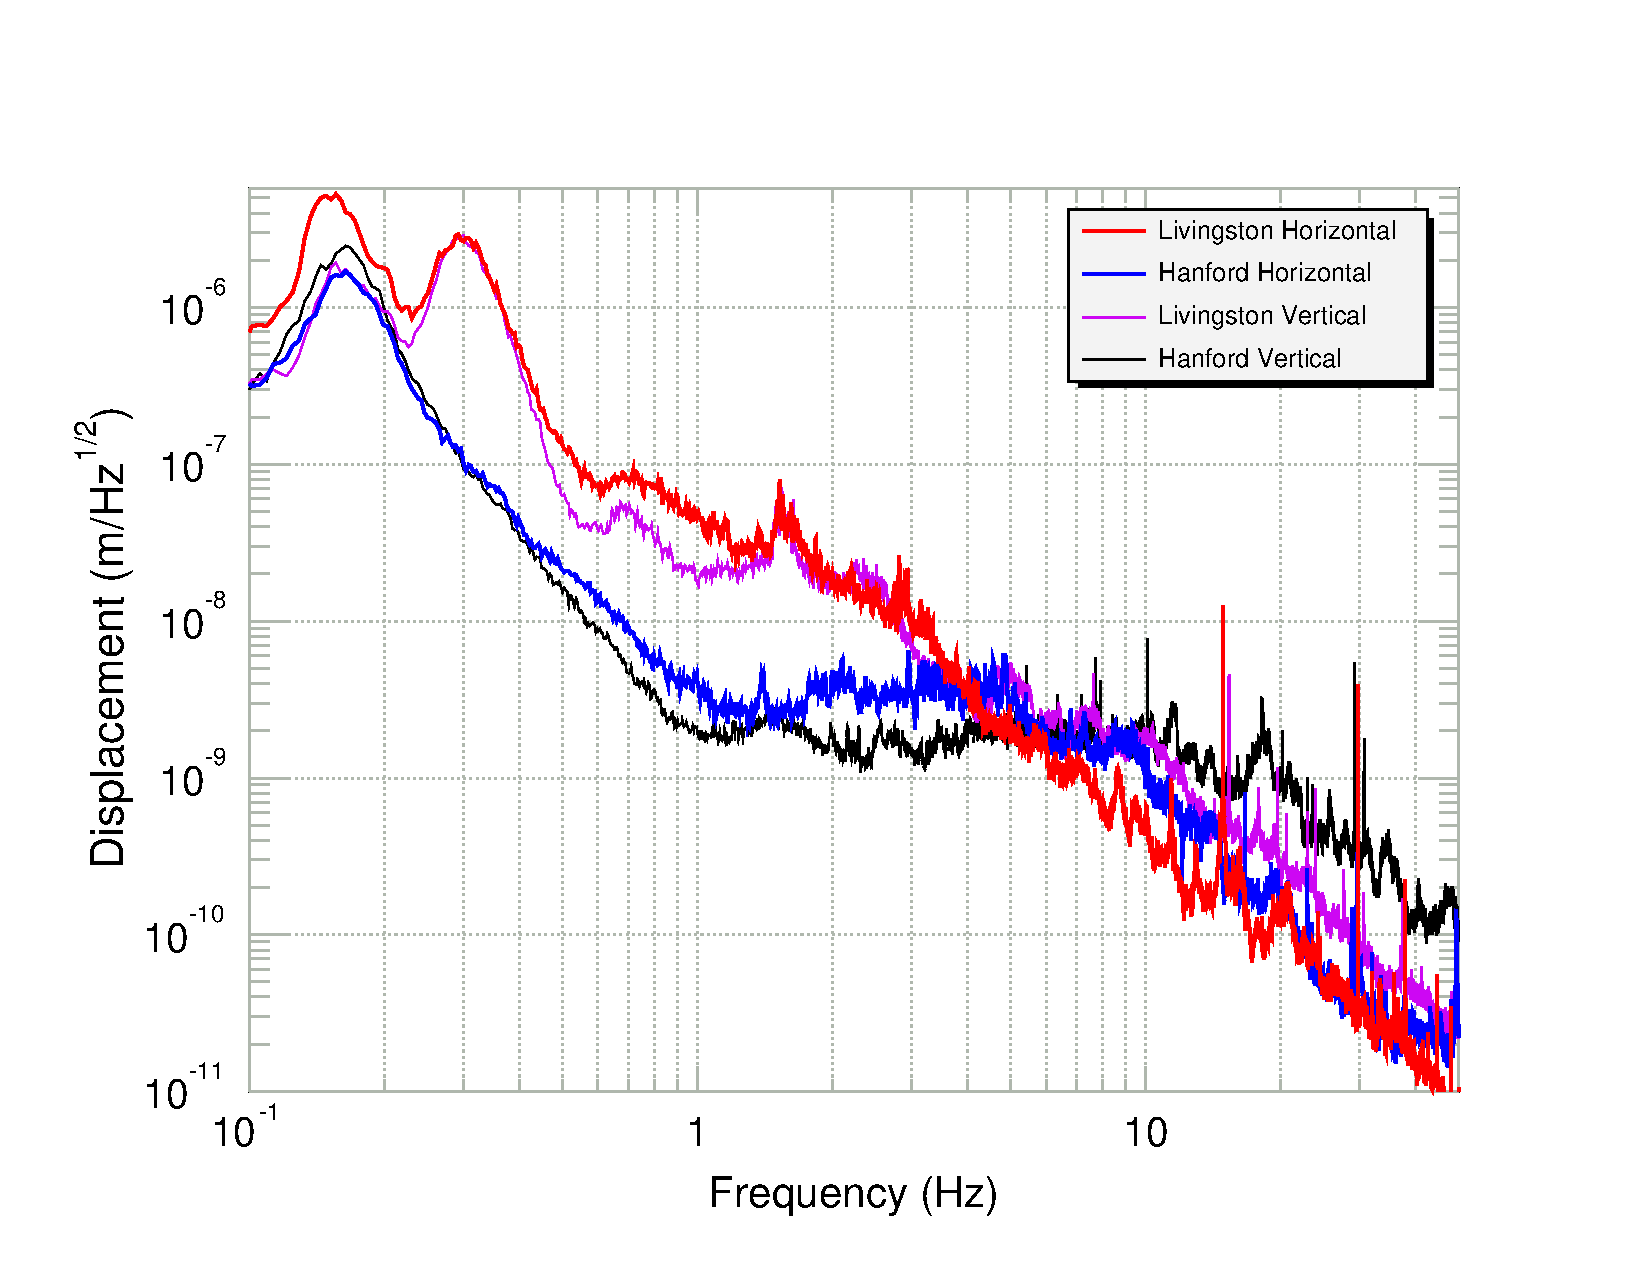
\includegraphics[angle=0,width=6.5in]{Figures/Chap4/LLOLHO-seis2.pdf}}
\caption[Seismic Spectra]{Amplitude spectral density of the daytime displacement 
                          noise of the ground at both LIGO sites.}
\label{fig:SeismicNoise}
\end{figure}

\subsubsection{Noise Characteristics}
\label{sec:SeismicCharacter}

\begin{itemize}
\item Excepting dramatic events such as earthquakes and subway cars, the largest
      ground motions seen everywhere are from the $\approx$6 second period 
      `microseism' \cite{useism}.
      The primary microseism is generated by ocean waves having a $\approx$12-15 second
      period. The secondary microseism, which is much larger, is produced
      by standing waves on land from a large number of sources.

\item The power in the 0.5-10 Hz band is largely due to man made noise. 
      The operation of the Livingston interferometer has been
      seriously impaired by this noise. The noise is so large that the
      interferometer only operates reliably from the end of the workday
      (6-8 PM on weekdays) until the beginning of the workday (5-6 AM).

\item Above 10 Hz, most of the noise is self inflicted. The acoustic and 
      vibrational environment at the observatories has been compromised 
      by the HVAC systems. 
      Efforts are underway to remediate this by balancing fans, installing 
      acoustic isolation and damping material, and isolating the noisiest components 
      with springs.
\end{itemize}


\subsubsection{Seismic Isolation}
To attenuate this noise, the core interferometer optics are each suspended
as pendula (see Section~\cite{sec:SUS}) by a single loop of steel wire. 
The pendulum length is set to put the resonant frequency 
to $f_{p} \simeq 0.75$ Hz. 
This reduces the coupling between ground noise and optic motion by 
$\sim(\frac{f_{p}}{f})^{2}$ above $f_p$.
\begin{figure}[!h]
\centerline{
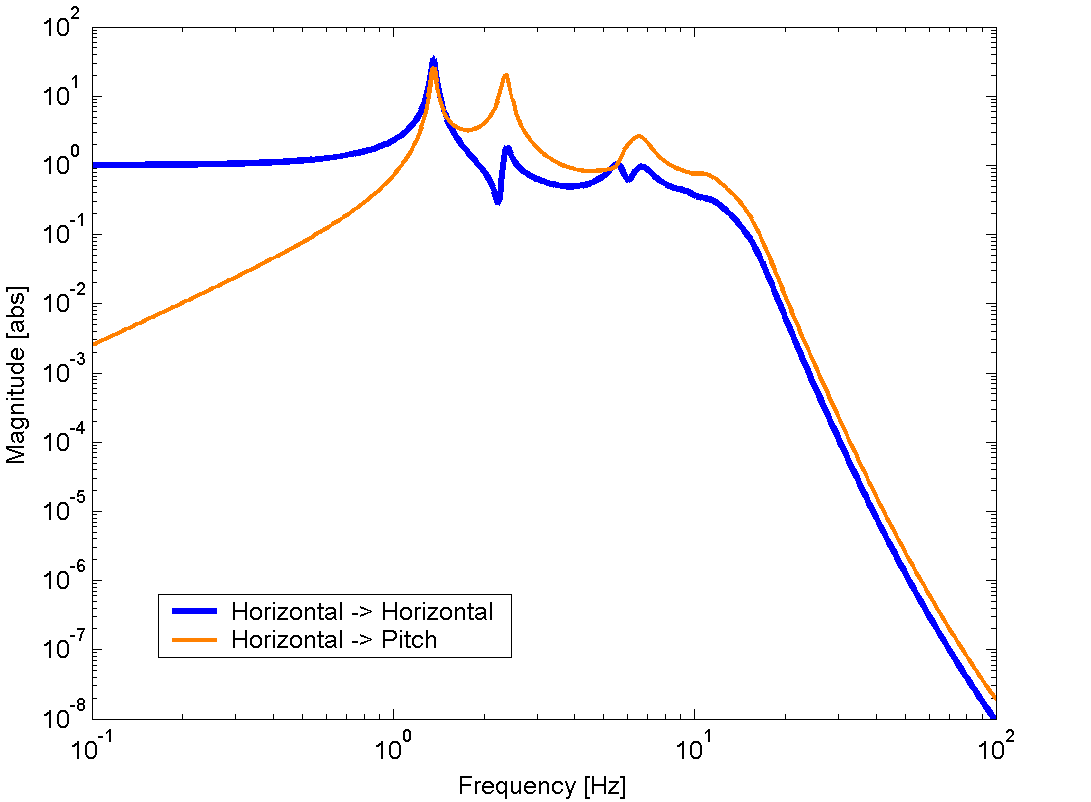
\includegraphics[angle=0,width=6.5in]{Figures/Chap4/BSCtf2.png}}
\caption[BSC Stack Transfer Function]{Modeled Isolation Stack Transfer Functions.}
\label{fig:StackTF}
\end{figure}
To get the rest of the required attenuation, the pendulum structure is placed upon
a stack of four alternating mass-spring layers (see Figure~\ref{fig:BSC}). Each of 
these layers gives another attenuation
factor proportional to $f^{-2}$, giving $\approx$100 dB of attenuation at 40 Hz and 
$>$140 dB at 100 Hz\cite{Giaime:ShitStack}.


%-------------------------------------------------------
\subsection{Thermal Noise}

At frequencies where seismic motion has been sufficiently filtered, the
interferometer's strain sensitivity will be limited by thermal noise.

The suspended mirror is in a radiative thermal equilibrium with the vacuum
chambers which are at room temperature. The thermal motions of the individual
particles of the glass, the mirror coating, and the mirror's suspension system
can cause fluctuations in the measured cavity length.

The reason that the thermal energy of the whole mirror / suspension system 
comes into play is that there is a coupling between all of the internal modes 
of the system and the motion of the mirror's surface. This coupling ensures 
that there is a continuous flow of energy between the degree of freedom we 
are trying to measure and all of the other internal degrees of freedom. 

The energy flow works both ways; the energy in one of the mirrors modes will
slowly dissipate as it couples into all the other modes. A general theme in
the thermal noise reduction game is reducing, as much as possible, all sources
of dissipation which damp motions \emph{in the degree of freedom we are
measuring}.

The relation between the amount of fluctuation of the mirror surface
and the dissipation in the system is described by the 
Fluctuation-Dissipation theorem\cite{Callen:FD}:

\begin{equation}
S_{x}(f) = \frac{k_{B} T}{\pi^{2} f^{2}} Re[Y(f)]
\end{equation}
where $S_{x}(f)$ is the power spectral density of fluctuations in a degree of
freedom $x$, $k_B$ is Boltzmann's constant, $T$ is the temperature of the system,
$f$ is the frequency of the motion and $Y(f)$ is the complex mechanical admittance 
(inverse of the impedance) of the system. One expression for admittance which 
is particularly useful is\cite{Saulson:Book}:

\begin{equation}
Y(f) = \frac{v(f)}{F_{therm}} = i \frac{2 \pi f \, x(f)}{F_{therm}}
\end{equation}
where $F_{therm}$ is the thermal driving force, $x$ is the readout variable,
and $v$ is the time-derivative of the readout variable.

In the case of a Fabry-Perot cavity, we are principally interested in one
degree of freedom: the one that makes a signal in our strain readout
channel. It takes a very special type of test mass motion to make it to
this signal port. Thermal fluctuations excite all of the internal degrees
of freedom of the mirror (pitch, yaw, roll, pringle), but most of these mirror 
surface motions only scatter light out of the cavity's fundamental mode 
into higher order modes which do not resonate in the cavity. The strain noise
that we measure comes from piston motions of the mirror along the cavity axis
(there are some small couplings between the degrees of freedom so in principle
we have to also ensure that the noise in the non-critical degrees of freedom is
not too large).

In the LIGO interferometers, we can separate the thermal noise sources into two
convenient categories: the fused silica mirrors which form the arm 
cavities and the steel suspension wire which supports the optics.

%-------------------------------------------------------
\subsubsection{Test Mass Thermal Noise}

The original estimates of test mass thermal noise made in the 20th century were
based on a normal mode decomposition of the optic's internal modes 
\cite{Fred:Thermal}. However, this method requires one to measure the
Q of every mechanical resonance up to $\sim$100 kHz in order to 
estimate the thermal noise accurately. A more direct approach described
by Gonz\'alez and Saulson\cite{Gaby:Acoustic}, applied to mirrors by 
Levin\cite{Levin:Thermal}, is to calculate the admittance for our 
readout variable, assuming a homogeneous loss in the bulk.

In addition to loss in the glass substrate of the mirror, loss in the dielectric 
coatings on the face of the optic\cite{Andri:Coatings} has been identified
as a significant source of thermal noise. Approximately 30 
alternating, 1/4 wavelength, layers of Ta$_{\mbox 2}$O$_{\mbox 5}$ 
and SiO$_{\mbox 2}$ are used to make the coatings. Although the amount of coating
material is small compared to the size of the mirror, its mechanical losses
are $\sim$1000 times greater than the fused silica substrate. 

The power spectral density of displacement noise for 
a single mass is \cite{Andri:Coatings}:

\begin{equation}
\label{eq:InternalThermal}
S_x(f) \simeq  \frac{2 \, k_B T}{\pi^{3/2} \, w \, Y_S \, f} \left[ \phi_S +
                   \frac{2 \, d_{\mbox{\tiny C}}}{\sqrt{\pi} \, w} \phi_C \right]
\end{equation}
The nominal values for these parameters are listed in Table~\ref{t:LOS}. Using the best
guess estimates at the time of this writing, the thermal noise from the substrate
is approximately the same as that from the coatings. The total substrate thermal noise
contribution from all four mirrors is:
\begin{equation}
\delta L_{-}(f) \simeq 5 \times 10^{-20} 
                  \left(\frac{100 \, \mbox{Hz}}{f}\right)^{1/2}
                  \left(\frac{\phi_S}{1 \times 10^{-7}}\right)^{1/2}
                  \frac{\mbox{m}}{\sqrt{\mbox{Hz}}}
\end{equation} 
The coating thermal noise contribution is:
\begin{equation}
\delta L_{-}(f) \simeq 2.5 \times 10^{-20} 
                  \left(\frac{100 \, \mbox{Hz}}{f}\right)^{1/2}
                  \left(\frac{\phi_C}{2 \times 10^{-4}}\right)^{1/2}
                  \frac{\mbox{m}}{\sqrt{\mbox{Hz}}}
\end{equation}
taking into account that the ETM coatings have almost twice as many layers as the
ITM. There are some indications~\cite{Gregg:Pie} that the intrinsic loss in fused
silica can be as low as 10$^{-8}$. If this turns out to be the case for the LIGO optics
then the total mirror thermal noise contribution to the interferometer strain noise
would be reduced by a factor of $\approx2$.

%-------------------------------------------------------
\subsubsection{Suspension Thermal Noise}
\label{sec:SUSthermal}
The core optics in the interferometer are each suspended by a single loop
of steel music wire, $\approx$0.3 mm in diameter. The thermal noise for the LIGO 
suspensions has been previously analyzed~\cite{Gaby:Thermal} using a full 6 
degree of freedom model of a mirror supported by an anelastic steel beam. 
The often used model for the loss is that of a frequency independent internal
friction. The following section compares the model predictions with the data 
from the interferometers.

As in the above case of test mess thermal noise, there are 2 pieces of
information needed to estimate the noise contribution: The transfer function
between force and test mass motion (the admittance) is one. The other is the
source term: in our case random thermal forces distributed over the suspension
structure.

The admittance is known and can easily be calculated numerically. The thermal
force distribution, however, depends on the loss distribution in the system.

One of the dirt effects in suspension thermal noise is excess loss introduced
at the suspension point \cite{Kovalik:Clamps}. This can 
come from rubbing due to improper clamping of the suspension 
wire~\cite{Kovalik:ClampSpeech}. This excess source of loss is difficult to
determine ahead of time and can best be established by in-situ measurements.
This was done by measuring the quality factors of the 'violin' modes of the
suspension wire in two ways:

First (the easiest way, after the fact) the power spectrum of the strain
channel was examined. Vibrations of the 
mass from the thermal fluctuations in the wire dominate the signal in the
340-360 Hz band. Due to slight asymmetries in the suspensions (such as wire
thickness, length and cross-sectional ellipticity), each side of
the wire loop has a slightly different frequency.

\begin{figure}[!h]
\centerline{
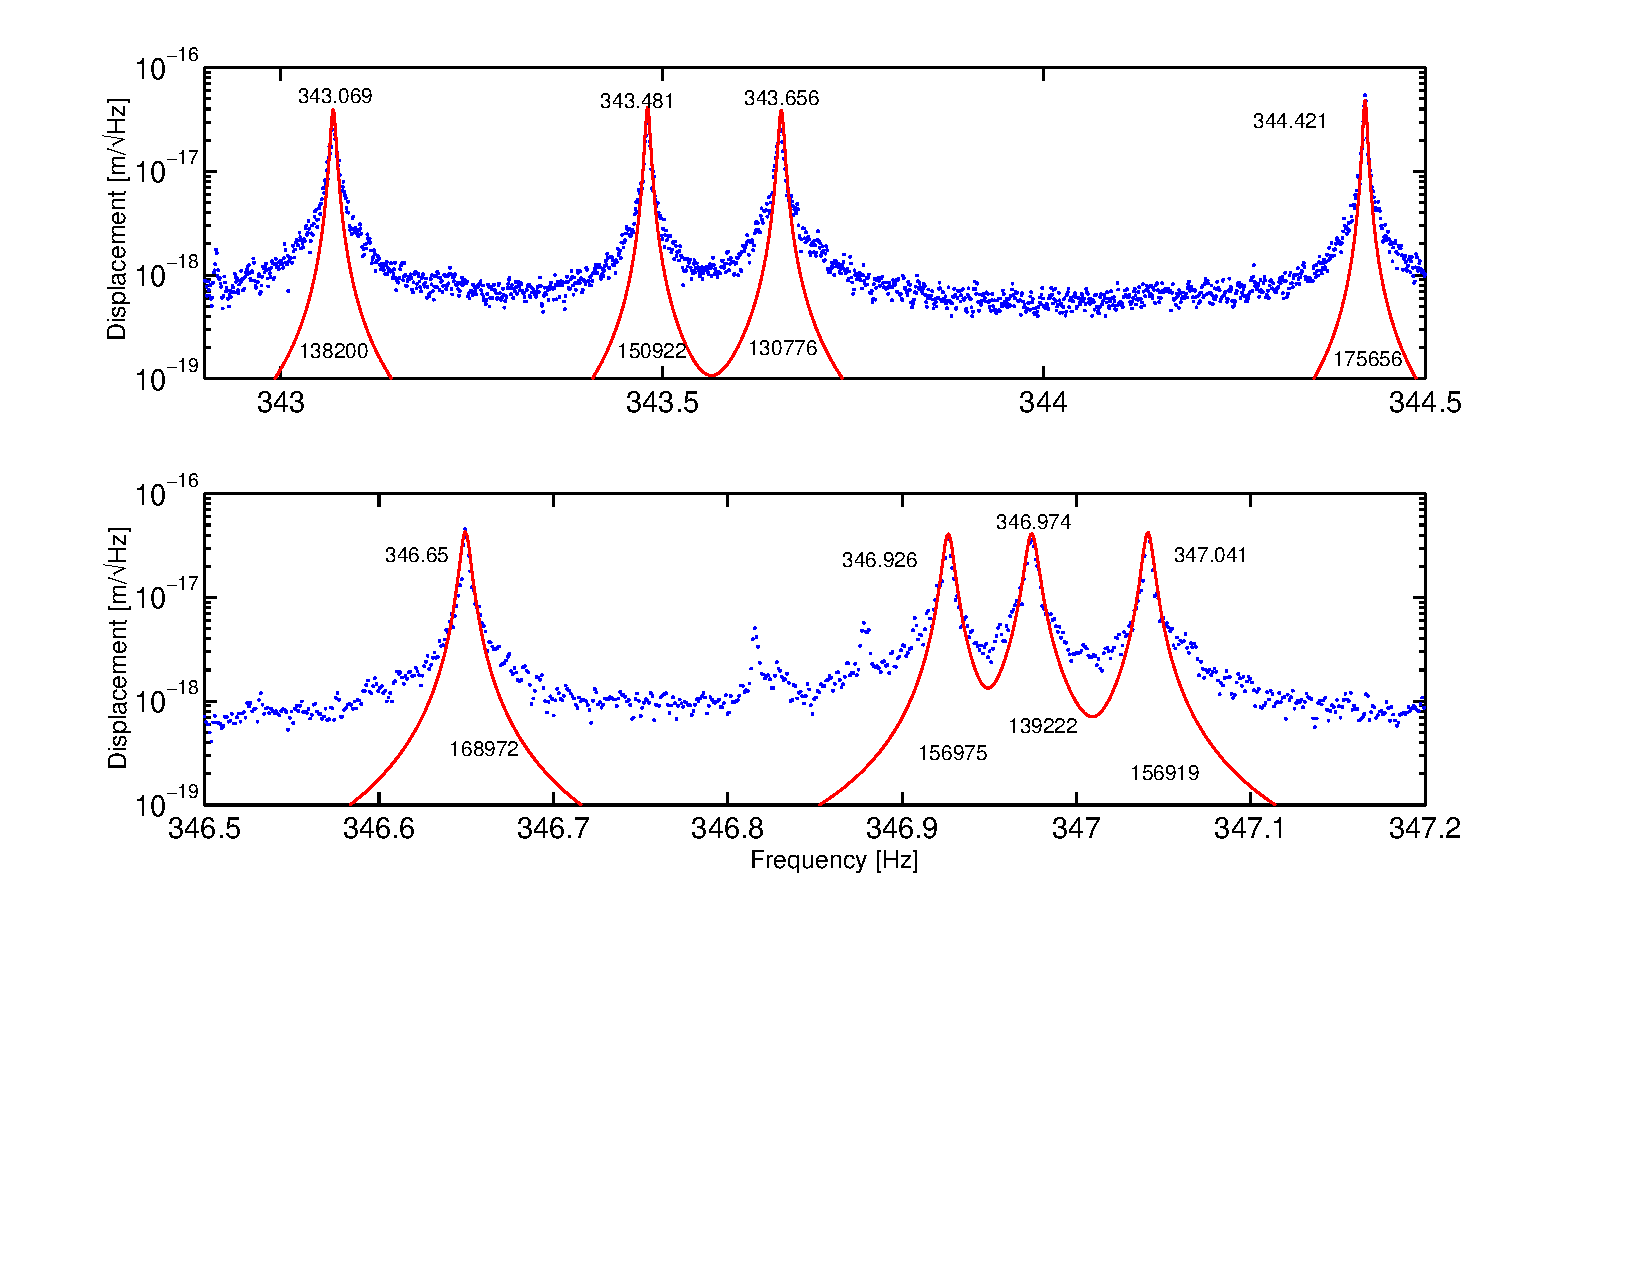
\includegraphics[angle=0,width=6.5in]{Figures/Chap4/violins.pdf}}
\caption[Violin Modes]{Displacement noise from the suspensions' violin
         modes. Plotted also is the fit to the data and the fitted
         frequencies and Q's.}
\label{fig:ViolinModes}
\end{figure}
A non-linear least squares fit to a Lorentzian curve was performed on each
peak. The frequency and Q from each fit is shown in Figure~\ref{fig:ViolinModes}.
Using the model from \cite{Gaby:Thermal}, we can place an upper limit on the average
loss angle for the violin modes of $\phi \lesssim 0.001$. From the fit we can see
that there is excess power in the wings of each peak; there is more than one
expects from a simple Lorenzian model for the peak. One possible source of this
excess noise is drift in the interferometer's optical gain on several minute
time scales. The next iteration of this measurement will have to use a gain corrected
displacement readout.


% Loss angle in steel:
% --------------------
% Virgo - C85 steel  1e-4
%
% Gaby - Paper       1e-3


Another weakness of this method is that it relies on several hours of
data in which the interferometer is assumed to be static. In reality,
a 1 degree C change in the temperature of the wire would result in a 10X
larger drift ($\approx$30 mHz) than what we are trying to measure.

To avoid the drift issues one would like to make a quick measurement.
One way is to measure the decay time for violin mode excitations
which only takes $\tau = Q/(\pi f_{vio}) \simeq 100$ seconds. This has the
drawback of interrupting science data taking but in principle has a much better
chance of success and should be pursued in the future to better estimate
the suspension thermal noise.


%-------------------------------------------------------
\subsection{Radiation Pressure}
\label{sec:radpress}

Technical radiation pressure noise comes from power fluctuations
of the input beam coupling to differential displacement noise through slight
asymmetries in the arms. Characterization of the LIGO optics (see \cite{COCwebsite}
and Appendix~\ref{app:optics}) allows us to estimate these couplings. 
Three sources of asymmetry are:

\begin{itemize}
\item Imbalance in the masses of the mirrors. ($\sim 0.3 \%$)
\item Imbalance in the arm cavity buildups. ($\sim 2 \%$)
\item The beamsplitter splitting ratio is not exactly 50/50. ($\sim 0.5 \%$)
\end{itemize}
For this noise to pose a problem, the power fluctuations on the input beam
must be rather high. Since the double cavity resonance attenuates all carrier
power fluctuations above 1 Hz, we find that in our signal band the contribution
is a few orders of magnitude below the sensitivity goal.


\subsubsection{Quantum Radiation Pressure}
Quantum radiation pressure, however, is not attenuated in this way. Quantum
mechanical radiation pressure noise in the interferometer comes from the
zero point fluctuations of the vacuum field which enters through the dark
port of the Michelson~\cite{Caves:RadPress}. A field which enters through the
dark port affects the two arms differentially. These fluctuations give rise to
a fluctuating force. The resulting displacement is:

\begin{equation}
x(f) = 2 \times \frac{2 \, \delta P}{m c (2 \pi f)^2}
                = \frac{1}{2 \pi^2 m c f^2} \sqrt{\frac{2 h c P}{\lambda}}
\end{equation}
The differential displacement for a nominal set of parameters is:

\begin{equation}
\Delta L_{-}(f) \thickapprox 10^{-22} \left(\frac{10.5 \mbox{kg}}{m}\right) 
                                      \left(\frac{100 \mbox{Hz}}{f}\right)^2
                           \left(\frac{P_{in}}{1 \mbox{W}}\right)^{1/2}
                            \frac{\mbox{m}}{\sqrt{\mbox{Hz}}}
\end{equation}
which is far below any reasonable estimate for the interferometer noise floor.


%-------------------------------------------------------
\subsection{Actuator Electronics Noise}

Usually when interferometer noise is described, things like
seismic, thermal, and shot noise are considered. As of this writing, the
noise source which has gotten the most work has been electronics noise in
the test mass actuator.

\begin{figure}[!h]
\centerline{
\includegraphics[angle=0,width=6.5in]{Figures/Chap4/actuation.jpg}}
\caption[Actuation Electronics]{The chain of digital and analog filters
         beginning with the pre-DAC whitening and ending with the box
         driving the current into the actuator coils}
\label{fig:OutputElectronics}
\end{figure}

The electronics which drive the test masses span the largest dynamic
range of any piece of electronics in the system. At the low frequencies it must correct
for the large ground fluctuations caused by storms and humans, whereas at
$\sim$100 Hz it must be quiet enough to not mask the gravitational wave
signals.

\subsubsection{Coil Driver}
\label{sec:CoilDriver}
The final electronics unit which drives the coils for the suspended optic
(described in Section~\ref{sec:OSEMdesc}) is called the coil driver.
There are 2 competing requirements on the coil drivers. They must have
a low enough spectral density of current fluctuations that this electronics
noise fall below other more fundamental noises (seismic, thermal). They
must also be able to provide enough force to acquire lock and maintain the
cavity resonance in the presence of large seismic disturbances.

The following figure shows how the low noise ({RUN} mode) and large range
{(ACQUIRE} mode) are accommodated.

\begin{figure}[!h]
\centerline{
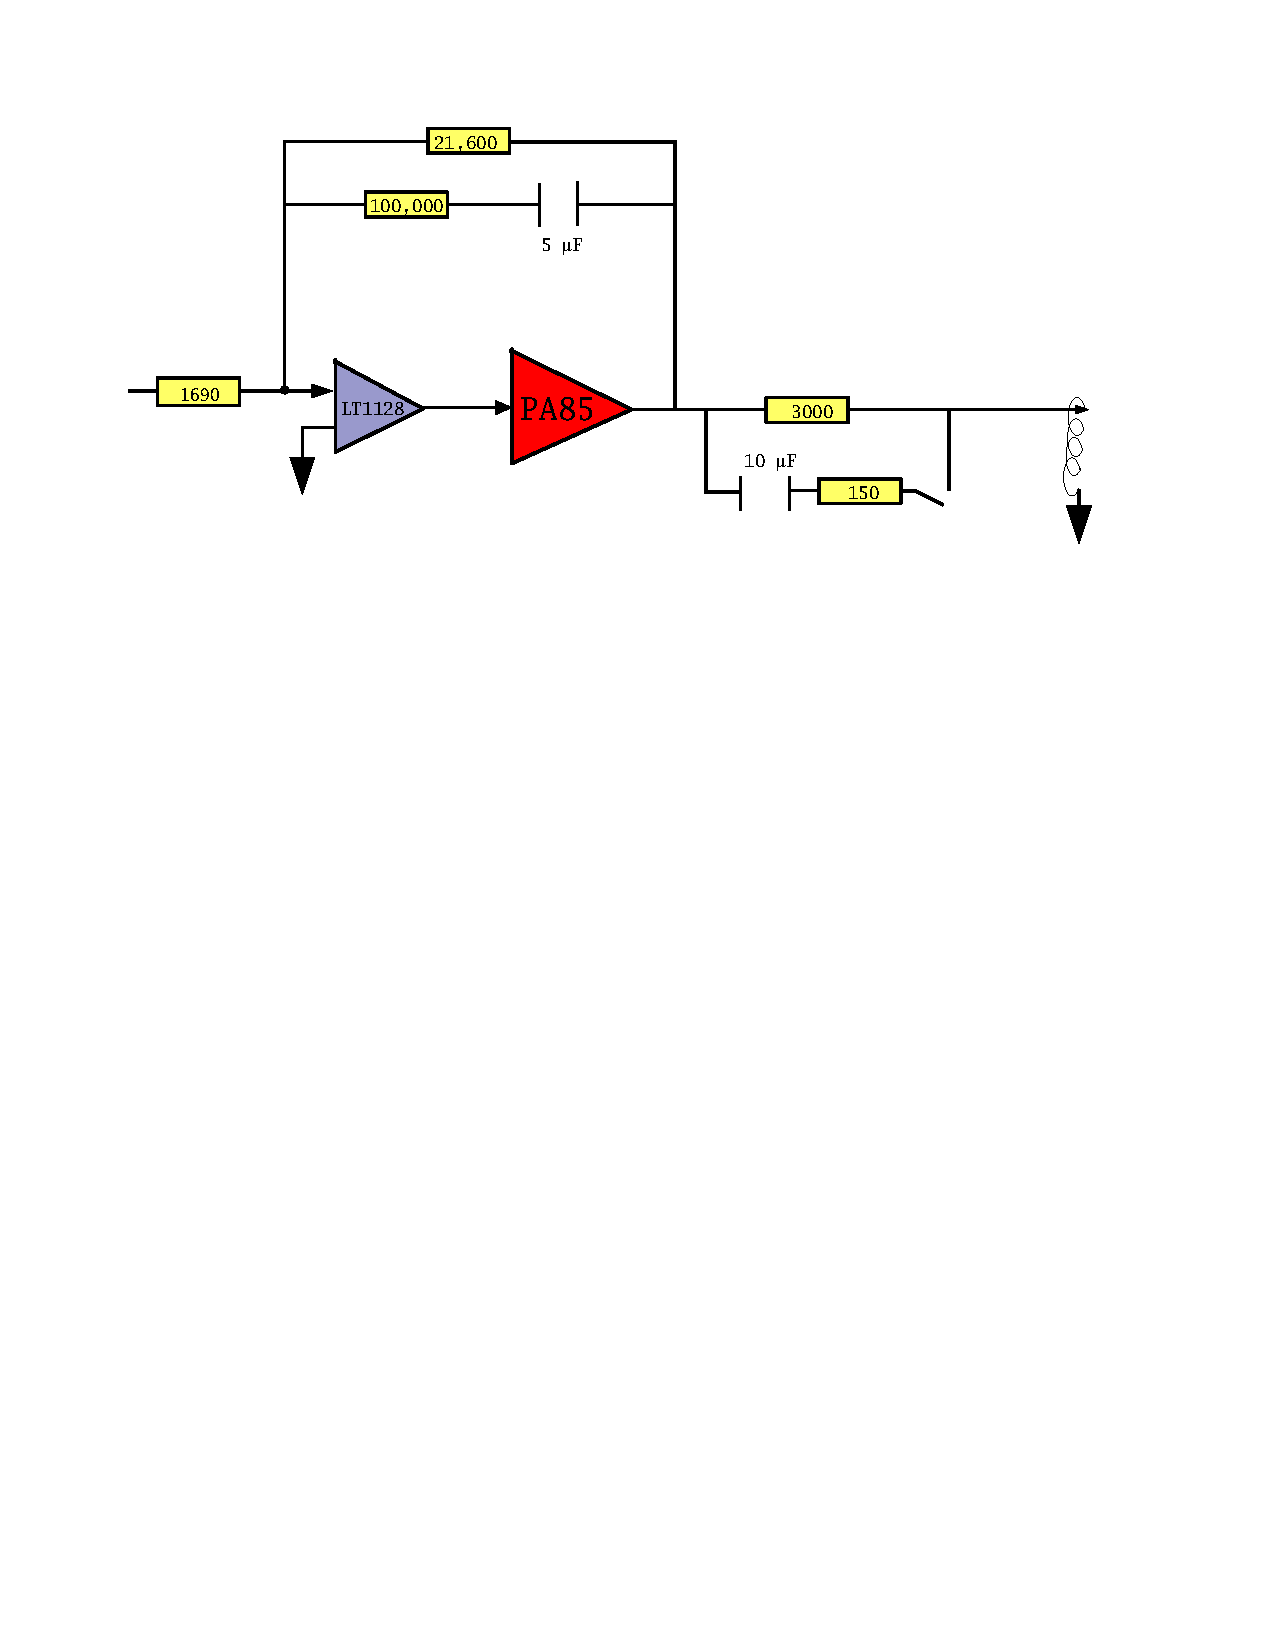
\includegraphics[angle=0,width=6.5in]{Figures/Chap4/coildriver.pdf}}
\caption[Coil Driver]{Simplified block diagram of the coil driver
         circuit for one face coil on one of the large optics. Closing
         the relay transitions from {RUN} to {ACQUIRE} mode. The yellow
         rectangles are resistors and the two spaced lines are capacitors.}
\end{figure}
A high voltage power amplifier (+/- 150 V, PA85) supplies current to the actuator coil
through a series resistor. In order to have a large dynamic range for lock
acquisition, a remotely controlled relay can engage a low impedance bypass
around the large series resistor. This gives a factor of $\sim$20 more force.

Since the servo system must hold the cavity within its narrow linewidth
during the switch a digital filter is employed to compensate the different
analog transfer functions. After acquiring lock the relay is switched
open and the digital compensation filter is turned off, leaving the
overall transfer function unchanged.

%The switching transient from this was large enough to move the 
%optic by $\sim$5 nm, breaking the lock. So a delay was


%-------------------------------------------------------
\subsubsection{DAC Noise}

Since the servo which controls the differential arm length is digital, the
drive signal to the coil driver must pass through a digital-to-analog
converter (DAC).

%The theoretical dynamic range for a DAC is:
%\begin{equation}
%V_{noise}(f)/\sqrt{Hz} = \frac{V_{p-p}/N_{bits}}{\sqrt{12 F_{s}}}
%\end{equation}

The LIGO DACs are 16-bit and have a 16384 Hz sampling rate. The dynamic
range (V$_{pp}$/V$_{noise}$(f)) is $\approx10^6$ in a 1 Hz bandwidth.

By contrast, the coil current spectrum must be able to supply 10 mA$_{\mbox{pk}}$ at
very low frequencies to accommodate the microseism and have a noise of less
than $10 \mbox{pA}/\sqrt{\mbox{Hz}}$ from 40-150 Hz. This gives a $\sim$1000X mismatch
in the dynamic range between the DAC and the optic's coil currents.

To satisfy both high and low frequency needs, an analog filter
is inserted between the DAC and the coil driver (the 'dewhitening' filter
of Figure~\ref{fig:OutputElectronics}). The filter has a unity gain
at low frequencies but then an attenuation of 4000 from 40-150 Hz. The
magnitude response of the filter is shown in Figure~\ref{fig:DWF}. Since
the current noise to displacement noise transfer function goes down
like $1/f^2$, the requirement on the coil current noise is much relaxed
above the target displacement noise minimum at 150 Hz.  
\begin{figure}[!h]
\centerline{
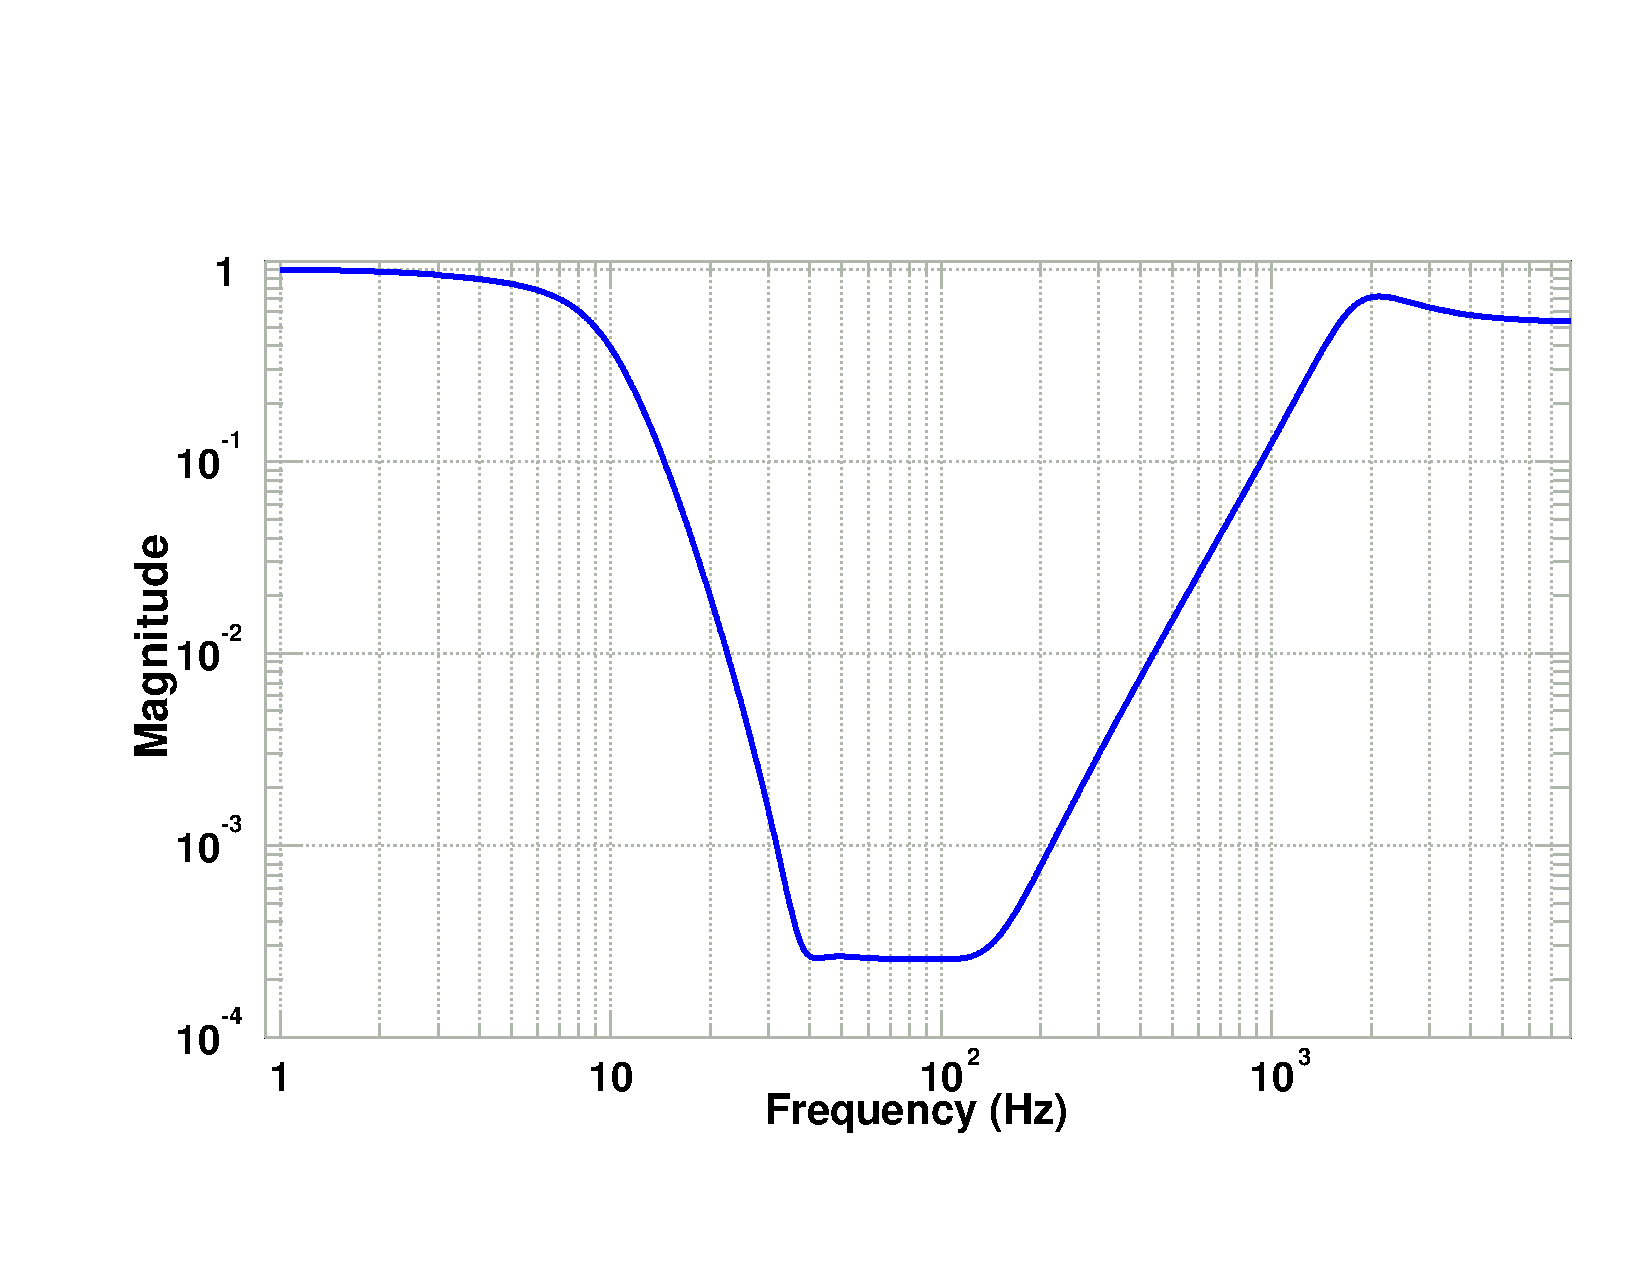
\includegraphics[angle=0,width=6.5in]{Figures/Chap4/dwf2.pdf}}
\caption[Dewhitening Filter]{Magnitude transfer function of the 
                             post-DAC dewhitening filter}
\label{fig:DWF}
\end{figure}
To keep the servo transfer function constant a digital inverse of
the analog filter is used to condition the signal before the DAC. There
is a potential for saturation in the DAC, due to the amplification in this
inverse filter. To reduce the dynamic range of the signal sent to the DAC,
the dewhitening filter is designed to only attenuate in the 40-150 Hz band
where the noise requirements are most critical.

\begin{figure}[!h]
\centerline{
\includegraphics[angle=0,width=6.5in]{Figures/Chap4/CoilNoise.pdf}}
\caption[DAC Noise]{A comparison of coil current noise from the electronics
         with the signal levels during S2. Also shown are the Johnson noise
         from a 3 k$\Omega$ resistor in series with the coil and the
         level of current noise required to meet the LIGO Science Requirement.}
\label{fig:OutputElectronics}
\end{figure}



%-------------------------------------------------------
\subsection{Angle to Length}

This section describes the mechanism for angular fluctuations of the optic to
affect the optical cavity length. The sources of angular fluctuations below
15~Hz are chiefly seismic. Above 15~Hz most of the angular noise comes from
the angular control servos (see Section~\ref{sec:ASC}).

The primary mechanism which couples angular noise into apparent length fluctuations
is the lever arm effect. If the beam is displaced from
the mirror's axes of rotation, a tilt will shift the phase of the entire beam
mimicking a length shift: $\delta x = d \, \tan{\theta}$, where $x$ is the translation
of the optic along the cavity axis, $d$ is the de-centering of the beam, and $\theta$
is the optic's rotation angle.

A second effect is cross-coupling of angular torque into piston motions of the optic
through imbalances in the magnets' dipole moments and the actuation electronics. 
The gravitational wave frequency band is far enough above the pendulum eigenfrequencies that 
we may treat the optic like a free mass. The torque applied by the control system is
$\mathfrak{T} = 4 F_c R/\sqrt{2}$, where $\mathfrak{T}$ is the torque, 
$F_c$ is the force per coil 
and $R$ is the radius of the optic. The displacement inducing force is 
$F_x = \alpha 4 F_c$, where $\alpha$ is the imbalance in the coils. The angle 
to length coupling may then be written as:

\begin{equation}
 \begin{aligned}
  \delta x &= \delta \theta \, \left [ \frac{F_x / m}{\mathfrak{T} / J} + d \right ]      \\
           &= \delta \theta \, \left [ \frac{\sqrt{2}}{4} \alpha 
               \left( R + \frac{H^2}{3 R} \right) + d \right ]
 \end{aligned}
\end{equation}
using the moment of inertia $J = \frac{1}{4} M R^2 + \frac{1}{12} M H^2$ for
a cylinder (see Figure~\ref{fig:SUS}).

In order to minimize the total noise, we adjust the coil gains individually to
minimize the overall angle $\rightsquigarrow$ length coupling for both pitch
and yaw rotations without regard to the actual mechanism. This method minimizes 
the noise at just one position on the mass, but can be done for whatever
position the beam is at. The alignment control system prevents long term
beam drift and so once optimized the noise should remain minimized.

The procedure to balance is to inject a sine wave into the 
pitch / yaw feedback path and then adjust the digital coil gains while reading 
back the response in the strain channel at the same frequency. We were able to 
automate this procedure and 
got an angle $\rightsquigarrow$ length coupling of 
$2 \times 10^{-4} \mbox{meters}/\mbox{radian}$; 
equivalent to a beam decentering of 0.2 mm or $\sim$0.3\% of a beam diameter. 
This level of balancing requires adjusting the coil gains at the 0.5\% level.

The obvious drawback to this method is that it does not actually center the
beam on the optic. Decentering can increase the sensitivity to thermal noise
in the suspensions angular eigenmodes (more on centering in Section \ref{sec:sweetspot}).

This method was not in place for the S2 run and so there the coupling was significantly
worse, $\approx0.1 \, \mbox{meters}/\mbox{radian}$.




%- - - - - - - - - -  -  -  - - - - - - -  -  -  -   -   -    -    -     -      -
%- - -  SENSING  NOISES- - - - - - -  -  -  -   -   -    -    -     -      -
%- - - - - - - - - -  -  -  - - - - - - -  -  -  -   -   -    -    -     -      -
\section{Sensing Noises}

Sensing noise includes noise which comes in on the laser, noise generated in the
interferometer (scattering), noise in the readout electronics, and shot noise from
the quantum statistics of the photons at the AS port. 


%-------------------------------------------------------
\subsection{Laser Amplitude Noise}
\label{sec:IntensityNoise}

Laser amplitude noise has three coupling mechanisms:

\begin{itemize}
\item Power fluctuations in the arms can produce differential lengths changes
      in the arm cavities if there is an imbalance in the stored power or
      the masses of the mirrors. As discussed above in 
      Section~\ref{sec:radpress}, this effect is negligible.

\item Power fluctuations in the mode cleaner can produce laser frequency
      noise through radiation pressure induced displacements of the low mass
      ($\sim$0.25 kg) MC mirrors. This is described in more detail in
      Appendix~\ref{app:ModeCleaner}.

\item Power fluctuations at the anti-symmetric port modulate the gain of
      the strain readout channel. Low frequency arm length fluctuations
      are upconverted into the gravitational wave band through this 
      amplitude modulation.
\end{itemize}
An input beam with low frequency amplitude modulation can be written as:

\begin{equation}
E_{in} = E_{0} \left(1 + \frac{\Delta A}{A} \right) \cos{\omega t} 
\end{equation}
where $A$ is the amplitude of the unmodulated laser light. The noise signal
in AS\_Q will by the multiple of two time series: $\delta G(t) \delta L_{-}(t)$. $G(t)$
is the optical gain at the AS port and $\delta L_{-}(t)$ is the $L_{-}$ servo's error point.

The coupling to the anti-symmetric port signal can be written as \cite{Sigg:FreqResp}:

% Intensity Noise Coupling
\begin{equation}
S_{\mbox{\tiny AS\_Q}} =
\aleph \, g_{cr} t_{sb} r_{c}' 
\left\{k \Delta L_{-} * 
\left[\frac{\Delta A}{A} 
\left(1 + \frac{1}{(1 + i f/f_{cc})(1 + i f/f_{c})}
\right) 
\right] 
\right\}
\label{eq:Intensity}
\end{equation}
where $*$ is the convolution of Fourier transforms of the two time series.
Above the double cavity pole, $f_{cc}$, the carrier fluctuations are filtered out
and so the optical gain modulation  comes from the amplitude noise on the RF sidebands which
travel unfiltered to the AS port.

Since laser amplitude noise is usually characterized by measurements of the power,
it is convenient to note that $2 \Delta A/A = \Delta P/P$. Another commonly
used expression for the power fluctuations is the Relative Intensity Noise (RIN)
which is equal to $\delta P_{rms}(f)/ P$.

Combining Equations \ref{eq:Intensity} and \ref{eq:darm2asq} we get
the apparent differential arm signal due to laser power fluctuations:

\begin{equation}
\delta L_{-}(f) = 5 \times 10^{-21} 
               \left[\left(\frac{\mbox{RIN}(f)}{1 \times 10^{-7}}\right) *
               \left(\frac{\Delta L_{-}(f)}{1 \times 10^{-13} \mbox{m}}\right)\right]
               \left(1 + \frac{f}{f_c}\right) \frac{\mbox{m}}{\sqrt{\mbox{Hz}}}
\end{equation}
Measurements of the intensity noise coupling have revealed that this bilinear
coupling term is dominated by a (currently) unexplained linear coupling which
is the equivalent of having a static $\Delta L_- \simeq 3 \times 10^{-13} \mbox{m}$.


%-------------------------------------------------------
\subsection{Laser Frequency Noise}
\label{sec:FreqNoise}

Fluctuations in the frequency of the laser can couple into
the interferometer's differential strain readout through imperfections in
the optics. The frequency noise of the laser is intrinsically limited by
spontaneous emission from the upper state into the laser mode. The spectral
density of the frequency fluctuations is given by
% Schawlow-Townes formula for laser frequency noise
\begin{equation}
\nu(f) = \frac{1}{2 \pi \, \tau_{st}} \sqrt{\frac{h\nu}{P_{laser}}} 
\end{equation}
which is a form of the Schawlow-Townes limit\cite{Yariv,Peter:YAG}.
Substituting parameters for the LIGO master oscillator give 
$\nu(f) \approx 30 \, \mbox{mHz}/\sqrt{\mbox{Hz}}$. In reality, the frequency noise
is dominated by technical noise (thermal, acoustic, electronics) below 100 kHz.

To achieved the necessary frequency stability the laser frequency fluctuations are 
suppressed by several stages
of active stabilization. This frequency stabilization scheme is detailed in
Section~\ref{sec:CMservo}. The following paragraphs mainly detail how the
unsuppressed frequency noise can couple into the strain readout.

Although there are multiple mechanisms for frequency noise to show up 
at the AS port, they have a common theme: an imbalance between the 
two arms of the interferometer spoils the otherwise perfect 
subtraction of laser noise.

To calculate the signal due to frequency noise, we write the 
laser frequency, $f$, as $f = f_{0} + \delta\! f_N cos(\omega t)$. 
Then the signal at the anti-symmetric port due to frequency noise is

% Frequency Noise Coupling Equation
\begin{equation}
 \begin{split}
S_{\mbox{\tiny AS\_Q}} = 
\aleph \, g_{cr} t_{sb} \frac{\delta\! f_N}{2 f} [
& 8 \pi \, r_{c} \frac{f_{c}l_{m}}{c} \frac{f}{f_{c}}
\frac{1 + i f / f_{c}}{1 + i f / f_{cc}} \\
+ &\frac{\delta f_{c}}{f_{c}} (1-r_{c}) 
\frac{f / f_{c}}{(1 + i f / f_{cc})(1 + i f / f_{c})} \\
+ &\delta r_{c} \frac{f / f_{cc}}{1+if /f_{cc}} ]
 \end{split}
\end{equation}
The first term in the above equation comes from the Schnupp asymmetry, 
$l_{-} \approx$ 175 mm. The audio-frequency, frequency noise sidebands on the
carrier light get different phase shifts in the two Michelson arms and so they 
do not perfectly cancel out at the AS port. This residual field beats with the
static sideband fields to produce a signal.

The second term is proportional to $\delta f_{c}/f_{c}$, the fractional
difference in the two arm cavity poles. For the 4 km arm cavities, 
$f_{c} \approx $ 85 Hz and the fractional difference has been
measured by cavity ringdown to be $\sim$2\% (see Appendix \ref{app:optics}). 
A mismatch in the arm cavity poles
comes about through a difference in the round-trip loss (including mirror
transmissions). The loss in the arms
is dominated by the $\sim$3\% transmission of the input test masses. Note that since
the end mirrors have a reflectivity of $\sim$1, an arm cavity with no internal
scatter loss or absorption will still have an overall reflectivity of $\sim$1. So
the carrier fields reflected from the two arms have the same amplitude, but
different phase. At frequencies above the arm cavity pole the carrier audio
sidebands do not resonate in the arms and so do not experience a differential
phase shift from the cavity pole imbalance. Therefore the frequency noise
coupling due to the arm cavity pole imbalance gets smaller above the arm cavity pole.

The third term in the equation is somewhat different and is, in practice,
the dominant effect. At frequencies
above the coupled cavity pole, the carrier's audio sidebands are filtered off
but the audio sidebands of the RF sidebands couple directly to the AS port.
In a perfect interferometer this would have no effect, but an imbalance in
the reflectivity of the arm cavities will produce a static, TEM$_{00}$ carrier
field at the AS port. Since the differential arm servo loop only suppresses
differential phase shifts, this static field is not nulled. The audio sidebands
of the RF sidebands then beat against this static carrier to produce a signal
in AS\_Q.

As shown in Figure~\ref{fig:FreqNoise}, the term from the reflectivity
imbalance is dominant. For typical parameters at frequencies above the arm
cavity pole the apparent displacement noise from frequency noise is:

\begin{equation}
\delta L_{-}(f) \simeq 3.5 \times 10^{-20} 
                  \left(\frac{\delta r_c}{5 \times 10^{-3}}\right)  
             \left(\frac{\delta f_N}{1 \times 10^{-6} \, \mbox{Hz}/\sqrt{\mbox{Hz}}}\right)
                  \frac{\mbox{m}}{\sqrt{\mbox{Hz}}}
\end{equation}

\begin{figure}[!h]
\centerline{
\includegraphics[angle=0,width=6.5in]{Figures/Chap4/FreqNoiseCoupling.pdf}}
\caption[Frequency Noise Couplings]{Shown are the three frequency noise
         coupling mechanisms. Asymmetries: $l_-$ = 175 mm,
         $\delta f_{c} = 2 \, \mbox{Hz}$, $\delta r_{c}$ = 0.5 \%}
\label{fig:FreqNoise}
\end{figure}
A reflectivity imbalance comes about through
a difference in the losses of the two arms. A full description of the 
optics' characterization is in Appendix~\ref{app:optics},
but stated simply, we know from the power buildup in the interferometer that
the scatter loss ($\approx$70 ppm/mirror) is more important than the ETM transmission
($\sim$10 ppm). 



%-------------------------------------------------------
\subsection{Oscillator Amplitude Noise}

A commercial signal generator (IFR 2023A) is used to generate the modulation
waveform for the resonant RF sidebands. The output of the oscillator is
multiply split; several outputs are used to power the local oscillator
input of the various mixers used to demodulate the RF signals from the
detection ports.

One output of the splitter is actively amplitude stabilized and then used
to drive a phase modulator (see Section~\ref{app:IOO}).
Residual fluctuations in the modulation amplitude lead to sideband
amplitude fluctuations. Noise on the amplitude of the sidebands
modulates the optical gain at all of the readout ports. The RF mixers 
which demodulate the RF signal from the photodiodes are driven to
saturation on the Local Oscillator (LO) port and so there is no sensitivity 
to amplitude fluctuations of the LO drives. 
Oscillator amplitude noise shows up as \cite{Sigg:FreqResp}

\begin{equation}
S_{\mbox{\tiny AS\_Q}} =
\aleph g_{cr} t_{sb} r_{c}' \frac{\Delta \Gamma}{\Gamma} \, k \Delta L_{-}
\end{equation}
where $\Gamma$ is the modulation depth in radians. At frequencies
above the arm cavity pole, for typical parameters we get:

\begin{equation}
\delta L_- \simeq 1 \times 10^{-19}
           \left(\frac{\Delta \Gamma(f) / \Gamma}{1 \times 10^{-7} /\sqrt{\mbox{Hz}}} \right)
           \left(\frac{f}{1 \, \mbox{kHz}} \right)
           \left(\frac{\Delta L_-}{1 \times 10^{-13} \mbox{m}_{\mbox{\tiny RMS}}} \right)
           \frac{\mbox{m}}{\sqrt{\mbox{Hz}}}
\end{equation}
The amplitude noise of the oscillator has been measured to be just below
10$^{-7}$ from 100-1000 Hz and falling rapidly above 1 kHz.



%-------------------------------------------------------
\subsection{Oscillator Phase Noise}

Another noise source is phase jitter on the oscillator. So far the exact
coupling mechanism of oscillator phase noise has not been determined
but measurements have been made which show that it is currently a limiting
noise source and so it pays to speculate about the coupling mechanism in
order to have some theory to test.

In principle, there is no first order coupling of oscillator phase noise
to the dark port since any noise is common to both the signal and the local
oscillator and is therefore canceled
in the demodulated signal. Relative phase lags in the two paths between
the oscillator and the mixer break this symmetry and can produce a sensitivity
to phase noise.

There are 3 main sources of phase lag:
\begin{itemize}
\item Relative path length differences lead to an overall time delay. The
      difference is $\sim30$ m. Although this gives a substantial
      phase shift at the modulation frequency, once this is compensated
      for (by e.g. a length of cable) the remaining phase shift at audio
      frequencies around the carrier are negligible: $\sim10^{-4}$ radians
      at 1 kHz.

\item The power recycling cavity has a pole frequency of 
      $\approx170 \mbox{kHz}$. This filters the phase noise on the
      optical RF sidebands, but does not affect the local oscillator
      and so makes a small differential phase shift proportional to
      $f$/(170 kHz) below the recycling cavity pole.

\item The dominant phase shift for the optical RF sidebands comes from the 
      mode cleaner which acts as a $\approx4$ kHz low pass filter on the
      phase noise.
\end{itemize}

Oscillator phase noise can be represented by modifying the expression
for the input field:

\begin{equation}
E_{in} =
E_{0} e^{i \Gamma cos(\omega_{m}t + \phi_{N} cos \omega_{a} t)}
\end{equation}
In principle, even with this asymmetry there would be no coupling. In
both the symmetric and anti-symmetric ports, however, there is a large
unsuppressed signal in the demodulation phase quadrature which is not
used in the interferometer length control (REFL\_Q \& AS\_I, respectively).
These large low frequency signals get mixed into the signal phase by the
fractional phase angle difference between the LO and RF paths.

The signal at the anti-symmetric port due to this signal can be written as:

\begin{equation}
S_{\mbox{\tiny AS\_Q}} =
S_{\mbox{\tiny AS\_I}} \frac{i f /f_{\mbox{\tiny MC}}}{1 + i f /f_{\mbox{\tiny MC}}} 
                       \phi_N(f) 
\end{equation}
The particular model of signal generator (IFR 2023A w/ option 14)
used to generate the modulation waveform was chosen because of its
low phase noise spectrum (-130 dBc/$\sqrt{\mbox Hz}$). Custom built 
quartz oscillators having phase noise as low as -160 dBc/$\sqrt{\mbox Hz}$ 
can be purchased, although the commercial signal generator allowed the kind
of frequency tuning flexibility which is outside the range of the
quartz oscillators. 

If it is true that the coupling mechanism depends on the amplitude of the
AS\_I signal, future reductions of the signal in this quadrature would also 
reduce the oscillator phase noise contribution to the strain sensitivity.



%-------------------------------------------------------
%\subsection{Scattering}
%
%Scattered light in the interferometer which returns to the anti-symmetric
%port photodetector can cause spurious signals. Some things which scatter:
%
%\begin{itemize}
%\item Rayleigh scattering off of the residual gas particles in the
%      long beamtubes. 
%
%\item Light which scatters unintentionally somewhere within the interferometer
%      and then returns to the main beam path can modulate the field at the
%      detection ports. Great care has been taken in the in-vacuum optical
%      layout to control all extra reflections of a significant level.
%      Backscattering of this type limits the sensitivity at the symmetric
%      port (see Section~\ref{sec:CMscatter}).
%\end{itemize}
%
%\subsubsection{Residual Gas}
%
%The scattering due to residual gas particles has the form \cite{Mike:Gas,Rai:Scattering}:
%
%\begin{equation}
%\delta L_{-}(f) = 4 \pi \alpha 
%      \sqrt{\frac{\rho}{v_{0}}\int\nolimits_{0}^{L_{0}}
%      \frac{exp[-2 \pi f w(z)/v_{0}]}{w(z)} \, dz}
%\end{equation}
%where $v_{0}$ is the mean particle speed, $w(z)$ is the beam radius,
%$\rho$ is the number density, and $\alpha$ is the polarizability.
%(need to get parameters for H2, H20, hydrocarbons)
%
%The noise from residual gas scattering is expected to be insignificant at
%our designed strain sensitivity level, due to very low pressure (column
%density) of the gas in the beam tubes.


\subsection{Beam Clipping on the Optical Tables}

As the sensitivity in the interferometers improved, it became clear that there
is a great deal of sensitivity to the acoustic noise on \emph{every} optical table.

This acoustic sensitivity comes about through clipping of the beam on the
optical table through apertures and dusty optics. A hypothesis is that
the large diameter junk fields, from the contrast defect for the carrier or
the instability of the recycling cavity for the sidebands, produce
a signal when clipped. The aperturing of the higher order fields produces
some light which overlaps with the TEM$_{00}$ mode to produce a signal. 

This is largely reduced by enforcing the standard practices
of cleanliness, careful alignment, and dumping of secondary beams (into beam
dumps which are dark at 1 micron). This type of noise is what was
mainly responsible for the 100-1000 Hz structure in the H1 and H2 curves in
Figure~\ref{fig:S2noiseComp}. It has been greatly reduced by the installation
of an acoustic isolation enclosure around the AS port tables
of each interferometer and by the use of larger optics on the table.



%-------------------------------------------------------
\subsection{Auxilliary Length Controls}
\label{sec:POBnoise}

Fluctuations of lengths other than the differential arm cavity
degree of freedom can produce signals at the Anti-Symmetric port. The average
length of the arm cavities is not controlled at most frequencies
but is tracked by the laser as described in Section~\ref{sec:CMservo}.

The other two lengths, $l_{-}$, the differential mode of the recycling
cavity and $l_{+}$, the common mode of the recycling cavity, produce
AS port signals in very different ways.

\begin{equation}
 \begin{split}
  \delta L_{-}(f) &= \frac{r_{c}}{r_{c}'} \delta l_- \\
                  &\simeq \frac{1}{140} \delta l_-
 \end{split}
 \label{eq:mich2darm}
\end{equation}
The $l_{-}$ coupling is straightforward; it is described by
Equation~\ref{eq:mich2asq}. The mechanism is similar to the way 
the differential arm signal is generated, the difference being that 
the $l_{-}$ signal does not get amplified by the arm cavity finesse.

\begin{equation}
 \begin{split}
  \delta L_{-}(f) &= 2 \delta r_{c} \frac{1}{r_{c}'} 
                     \frac{g_{sb} r_{M}}{t_{RM} t_{M}}
                     \delta l_{+} (1 + i f / f_c) \\
           &\simeq \frac{1}{1400} \delta l_{+} (1 + i f / f_c)
 \end{split}
 \label{eq:prc2darm}
\end{equation}
The $l_{+}$ coupling turned up unexpectedly in the course of 
commissioning. It is produced in a similar way to laser 
frequency noise coupling: audio sidebands on the RF sidebands beat with a 
static carrier at the AS port to produce an audio frequency signal. 
In this case, the audio sidebands are created by modulation of 
the $l_{+}$ length. The static carrier is produced by a reflectivity
imbalance between the two arms, same as frequency noise coupling.

\begin{figure}[!h]
\centerline{
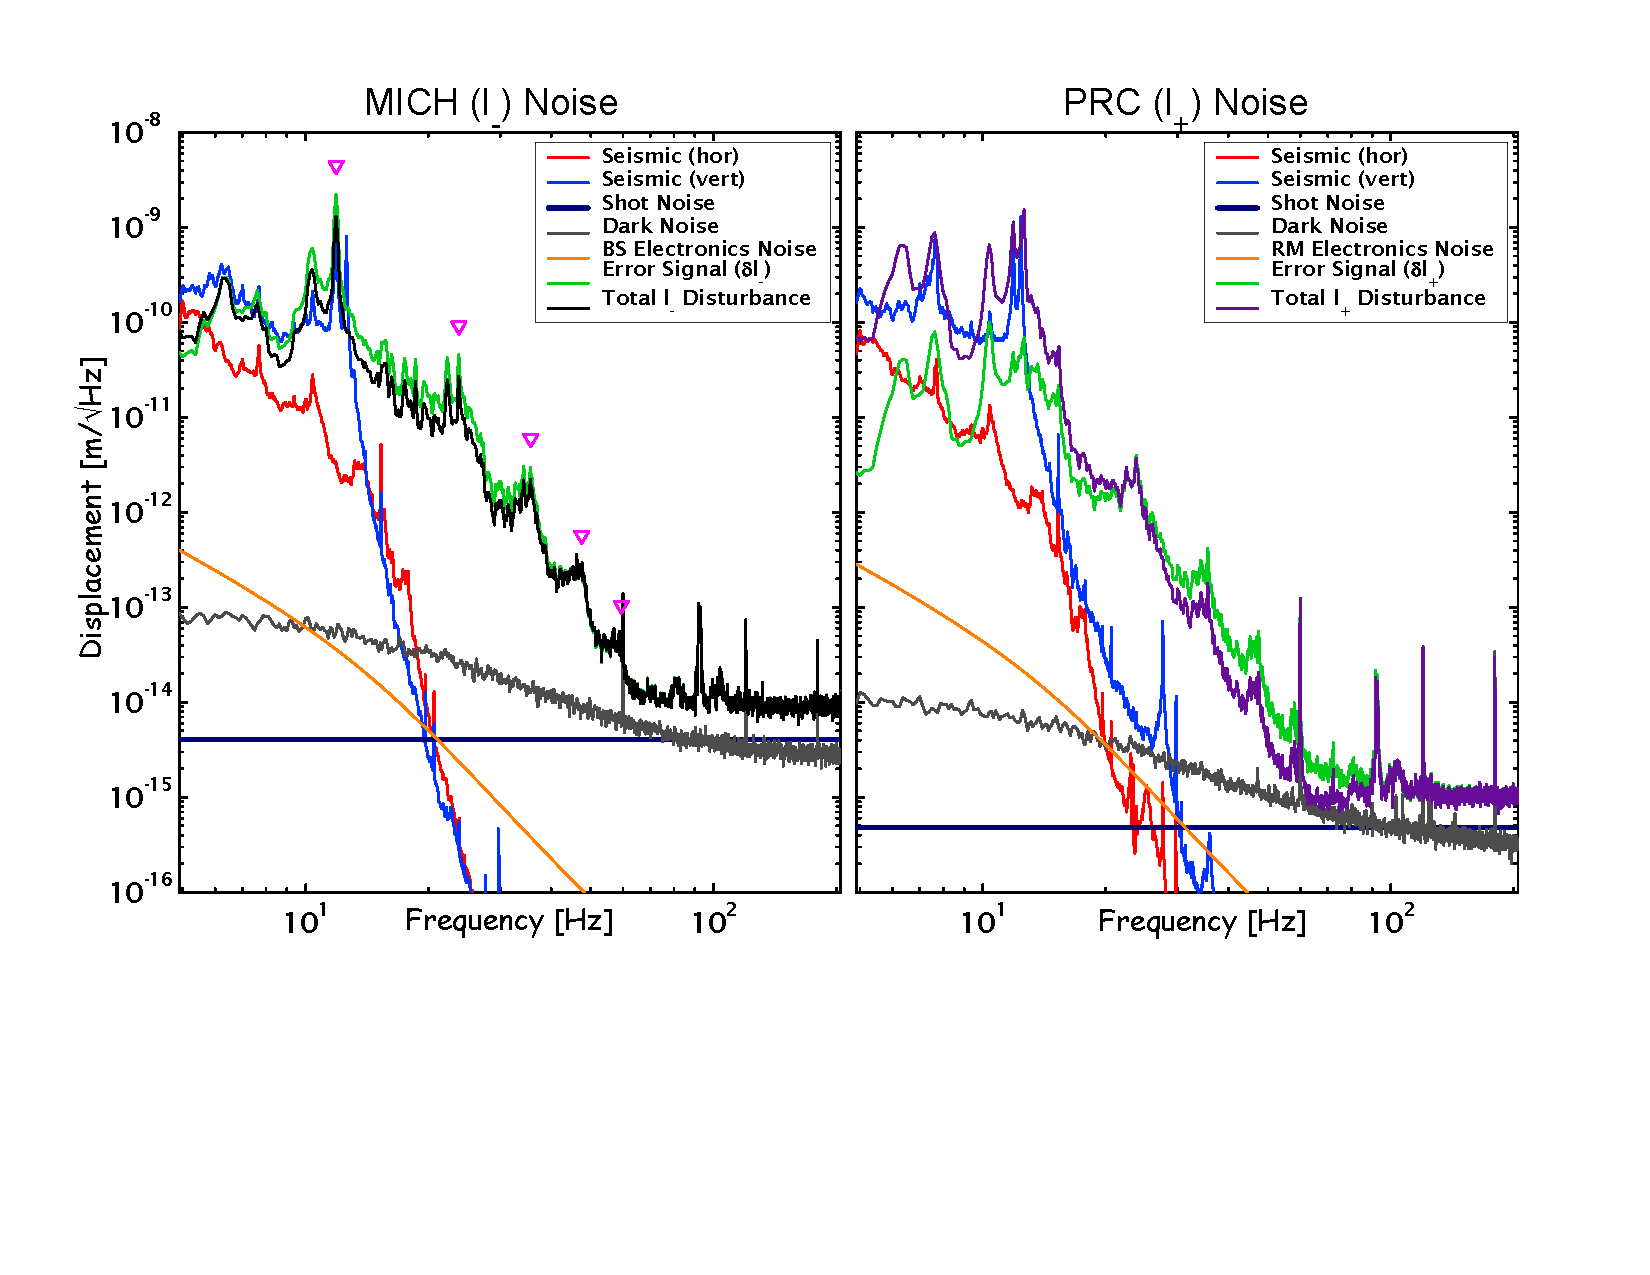
\includegraphics[angle=0,width=6.5in]{Figures/Chap4/POBnoise.pdf}}
\caption[POB Noises]{The two plots show the displacement
         spectra for both of the recycled Michelson DOFs; MICH ($l_-$) 
         \& PRC ($l_+$) and their known contributing noise sources.
         The triangles on the MICH plot indicate the harmonics of
         suspended optic's vertical bounce mode.}
\label{fig:POBnoise}
\end{figure}

Both of these lengths must be controlled in order to keep the interferometer
resonating. The length controls servos' gain must also be high enough
that the residual fluctuations of these lengths do not compromise the
strain sensitivity (more on this in \ref{sec:LSC}).

The largest disturbance to these lengths comes from seismic noise. As
shown in the plots, the dominant contribution is from vertical noise.
The 'vertical noise' traces actually refer to the apparent cavity
length fluctuations which arise from vertical motion of the optic.

The coupling is much larger for the recycling cavity than for the
arm cavities. In this case, the $\sim$1 degree vertical wedge angles
are the main coupling source. The exact positions and angles
of each optic surface are documented \cite{Dennis:WedgeAngles}. The
'vertical noise' trace is estimated by first measuring the vertical
motion with an accelerometer mounted external to the vacuum chamber.
This trace is converted into displacement units, multiplied by
the modeled vertical $\Rightarrow$ vertical transfer function of the 
stack, and then multiplied by the vertical $\Rightarrow$ vertical transfer function 
of the pendulum suspension which takes into account the compliance 
of the steel suspension wire.

This is done separately for each of the four recycling cavity masses and
then summed with the appropriate geometrical factors to make the displacement
noise.

In principle, the only other noise limit to these lengths should be
in the sensing chain. The dark noise curve in Figure~\ref{fig:POBnoise}
is the result of ADC noise below 100 Hz and the noise of the photodetector
above 100 Hz. The shot noise limited displacement sensitivity of these
degrees of freedom is rather high compared to the Anti-Symmetric or
Reflected ports; only a small fraction
of the circulating field  in the recycling cavity is picked-off for the 
signal detection.

It is clear from these plots, that the normal linear coupling mechanisms
are not good enough to predict the noise that we actually see. The 
indicators in the MICH plot of Figure~\ref{fig:POBnoise} show what appears
to be significant upconversion of the large amplitude low frequency 
motions, implying that the bilinear noise mechanism has, as one of its
terms, the vertical bounce mode.



%-------------------------------------------------------
\subsection{Shot Noise}
\label{sec:ShotNoise}

Vacuum field fluctuations entering the interferometer through the
anti-symmetric port affect the interferometer's phase sensitivity
by beating with the RF sidebands~\cite{Caves:RadPress,Caves:Squeezing}. 
This is often described
as 'shot noise': Poisson arrival time statistics of the light
on the photodetector.

In addition to this more fundamental noise source, there is also extra
shot noise introduced by the presence of junk light on the photodiode.
The differential arm signal is in principle only dependent on
the amount of light in the TEM$_{00}$ mode but the shot noise level
depends on the total light level since the light power level is not
dominated by the beat between the carrier and sideband fields.

The expression for the shot noise signal at the AS port is\cite{Sigg:FreqResp}:

\begin{equation}
S_{\mbox{\tiny AS\_Q}} =
2 \sqrt{[J_0(\Gamma)^2 g_{cr}^2 c_d 
       + \frac{3}{2} 2 J_1(\Gamma)^2 t_{sb}^2] P_{in} h \nu}
\label{eq:ShotNoise}
\end{equation}
where $c_d \equiv P_{AS}/P_{BS}$ is the carrier contrast defect. 
The two terms in the bracket are essentially 
just the carrier power 
($\propto J_0(\Gamma)^2$) and the sidebands' power ($\propto J_1(\Gamma)^2$). The
factor of 3/2 in the term for the sidebands' power derives from the non-stationary
nature of the shot noise produced by the 
sidebands~\cite{Niebauer:ShotNoise} and the fact that we are using
effectively a sine wave demodulation~\cite{Meers:modulation}.
Combining Equations \ref{eq:darm2asq} and \ref{eq:ShotNoise} gives us an 
expression for the equivalent differential arm length noise:

\begin{equation}
\delta L_- \simeq 3.6 \times 10^{-17} \sqrt{\frac{1}{P_{in}}}
            \frac{\sqrt{J_0(\Gamma)^2 g_{cr}^2 c_d 
                     + \frac{3}{2} 2 J_1(\Gamma)^2 t_{sb}^2}}
                 {J_0(\Gamma) J_1(\Gamma) g_{cr} t_{sb} r_{c}'}
             \left(1 + i \frac{f}{f_c}\right)
            \frac{\mbox{m}}{\sqrt{\mbox{Hz}}}
\end{equation}
We can then optimize the SNR, by adjusting the modulation depth, $\Gamma$,
to minimize this function.


\subsubsection{Mode Overlap and Optical Gain}

The above formula and all of the formulae in Chapter~\ref{chap:signals}
are valid in the limit that all of the light is in the same spatial
mode. This is not exactly true at any port; the situation at the
Anti-Symmetric port is of the most concern.

The differential arm strain signal is encoded on the carrier light
returning to the beamsplitter as a differential phase shift. After
interfering at the beamsplitter a small field proportional to this
phase difference comes out of the AS port. The spatial
profile of this signal field is set by the \emph{average} of the
resonant modes in the two arm cavities. If the arms
are well matched spatially, this is not a significant distinction
to make.

What is significant is the spatial mode of the RF sidebands at the
AS port. Due to the spatial mismatch between the
recycling cavity 'mode' and that of the arm cavities
(see Section~\ref{sec:ThermalComp} for details), some fraction
of the sideband field at the AS port contributes to making
shot noise but not to the signal gain.

Nominally, the length signal, AS\_Q, is not sensitive to the higher
order spatial modes except as it relates to the generation of shot noise.
This is because a higher order TEM$_{mn}$ mode is orthogonal to the
nominally TEM$_{00}$ local oscillator field of the RF sidebands.
However, the presence of higher order modes in both the sidebands and
carrier will contribute directly to the signal (some in AS\_I
and some in AS\_Q). This signal is nulled in the I-phase quadrature
with the AS\_I servo (see Section~\ref{sec:Gorilla}), but in the
Q-phase this signal has to be nulled by introducing a differential
arm length offset.



%-------------------------------------------------------
\subsection{Readout Electronics}

Another technical source of noise is the electronics chain which reads
out the strain signal. The following block diagram shows the signal flow:

\begin{figure}[!h]
\centerline{
\includegraphics[angle=0,width=6.5in]{Figures/Chap4/SensingChain.jpg}}
\caption[Sensing Electronics]{Shows the signal flow from the RF photodiode to
         the analog-to-digital (ADC) converter.}
\end{figure}

Since the goal is to achieve the minimum strain noise possible we design
the electronics noise to be less than 1/10 of the noise coming from the more
fundamental shot noise.

To accomplish this, the signal-to-noise ratio achieved at the front end
electronics is not degraded throughout the chain into the ADC. The 
dark noise of the photodetector at the anti-symmetric port (described in 
more detail in Appendix~\ref{app:RFPD}) is in principle, \emph{dominated by the 
thermal noise of the LC resonant circuit formed by the photodiode and the inductor}.
So the requirement on the whitening electronics is only to increase the
signal from shot noise (or other 'fundamental' sources like thermal or seismic)
to at least 10X the ADC noise level. This is balanced by the desire to maintain 
a factor of 30 or more in headroom between the RMS signal level and the ADC input range.



%- - - NOISE NOISE NOISE NOISE - - - - - - -  -  -  -   -   -    -    -     -      -
\section{Some Notes about the Noise}

The interferometer noise is usually unexplained in several frequency bands and 
it is always changing (sometimes for the better). Therefore,
I have attempted here to give a good accounting of the noise as it was in
2002-2003, which were the years in which LIGO held its first three science runs
(creatively named S1, S2 \& S3).

\subsection{The Status of the Noise}

\begin{figure}[!h]
\centerline{
\includegraphics[angle=-90,width=6.5in]{Figures/Chap4/S3noise.pdf}}
\caption[S3 Noise]{Full Noise Budget for L1 during S3 (data from Dec. 23, 2003)}
\label{fig:S3noise}
\end{figure}
Figure~\ref{fig:S3noise} is a good summary of this entire chapter. The point of
doing all of the noise analysis and budgeting is to always know what noise
sources limit the interferometer sensitivity and how this noise can be reduced.
The traces in the plot are not all made in the same way. Some of the traces
(e.g. oscillator phase noise) are made by measuring the source of the noise
(oscillator phase noise) and then the transfer function to AS\_Q and then 
multiplying them. Other traces
(e.g. internal thermal noise) are almost entirely based on a model for the
noise with few measurements for support.

The noise will often fluctuate upwards by factors of a few due to short time
transients or instabilities in the control servos. These plots of the amplitude
spectral density do not capture this character.


\subsection{A Brief History of the Noise}

These interferometers actually 'awoke' with noise levels at least 5 orders
of magnitude higher. These next paragraphs attempt to give a short synopsis 
on the major developments between each noise epoch shown 
in Figure~\ref{fig:NoiseHist}.

\begin{figure}[!h]
\centerline{
\includegraphics[angle=-90,width=6.5in]{Figures/Chap4/NoiseHist.pdf}}
\caption[LLO Noise History]{Noise history of the Livingston Interferometer from
                            2001-2003.}
\label{fig:NoiseHist}
\end{figure}


\subsubsection{May 18$^{th}$, 2001}

Pre power-recycling. The RM is misaligned intentionally to allow locking of
the Fabry-Perot Michelson in an optically recombined but not recycled mode. 
In this configuration there is very little
light at the anti-symmetric port available for locking and so the noise above
1 kHz is dominated by the dark noise of the sensing electronics. The vast array
of line spikes at multiples of 60 Hz are from the switching power supplies which were
in use at this time. In addition, there is no feedback from the interferometer 
to suppress laser frequency noise which therefore dominates the noise from 80-500 Hz.


\subsubsection{December 12$^{th}$, 2001}

The vacuum system was vented over the summer of 2001 to allow a number of repairs:
several of the suspensions' local sensors had broken photodiodes, wires, etc. 
In addition this version of local sensor had a photodiode which was sensitive to 
the 1064 nm laser light. New sensor / actuator heads were installed on all optics 
which are more than 100X less sensitive at 1064 nm.


\subsubsection{December 21$^{th}$, 2001}

Lower DAC Noise: First successful attempts to run the interferometer with the 
post-DAC dewhitening filters.


\subsubsection{May 27$^{th}$, 2002}

Power recycling and frequency stabilization. The first part of this year
was spent increasing the robustness of the the power-recycled configuration. 
The common mode servo was installed in a preliminary configuration and gave some
suppression of the frequency noise.


\subsubsection{August 24$^{th}$, 2002  (S1 Science Run)}

Common mode servo was revamped: $L_+$ feedback to the arms was removed
and the CM feedback to the mode cleaner length was changed to use a digital
servo. At this point it was discovered that through some non-linear
mechanism the noise is AS\_Q around 100 Hz could be reduced by increasing
the differential arm loop gain at 10-20 Hz. This later turned out to be
large bilinear upconversion around the power line harmonics. The source
was never identified, but the noise went away in the next major 
electronics upgrade.


\subsubsection{March 6$^{th}$, 2003  (S2 Science Run)}

All the electronics for the suspension controls are replaced with a mostly digital 
system allowing for greater flexibility. The introduction of the AS\_I servo
made it possible to detect nearly all of the light at the anti-symmetric port.
The large shelf of noise at 35 Hz from the optical lever servos is finally
reduced by whitening the optical lever sensor signals before the ADC.


\subsubsection{December 24$^{th}$, 2003  (S3 Science Run)}

Very little broadband improvement in sensitivity. An acoustic enclosure
was installed over the anti-symmetric port optics table, greatly reducing the
acoustic noise susceptibility. Efforts to commission the wavefront sensor
based angular control system were only partially successful and most of the run
had only 8 out of 16 degrees of freedom under control; 6 more than in S2, but not
enough to greatly improve stability.

The noise improvements at low
frequencies came from improved filtering of the optical lever servos
and the Michelson control loops. One notable improvement is the addition
of an off diagonal drive in the length control which feeds a small
fraction of the $l_-$ control signal to the $L_-$ length. This was
implemented mid-run and greatly improved the character of the noise
in the 30-70 Hz region.


\begin{figure}[!h]
\centerline{
\includegraphics[angle=0,width=6.5in]{Figures/Chap4/S1noiseComp.pdf}}
\caption[S1 Noise Curves]{Comparison of the interferometer noises during the
           first Science Run (S1).}
\label{fig:S1noiseComp}
\end{figure}


\begin{figure}[!h]
\centerline{
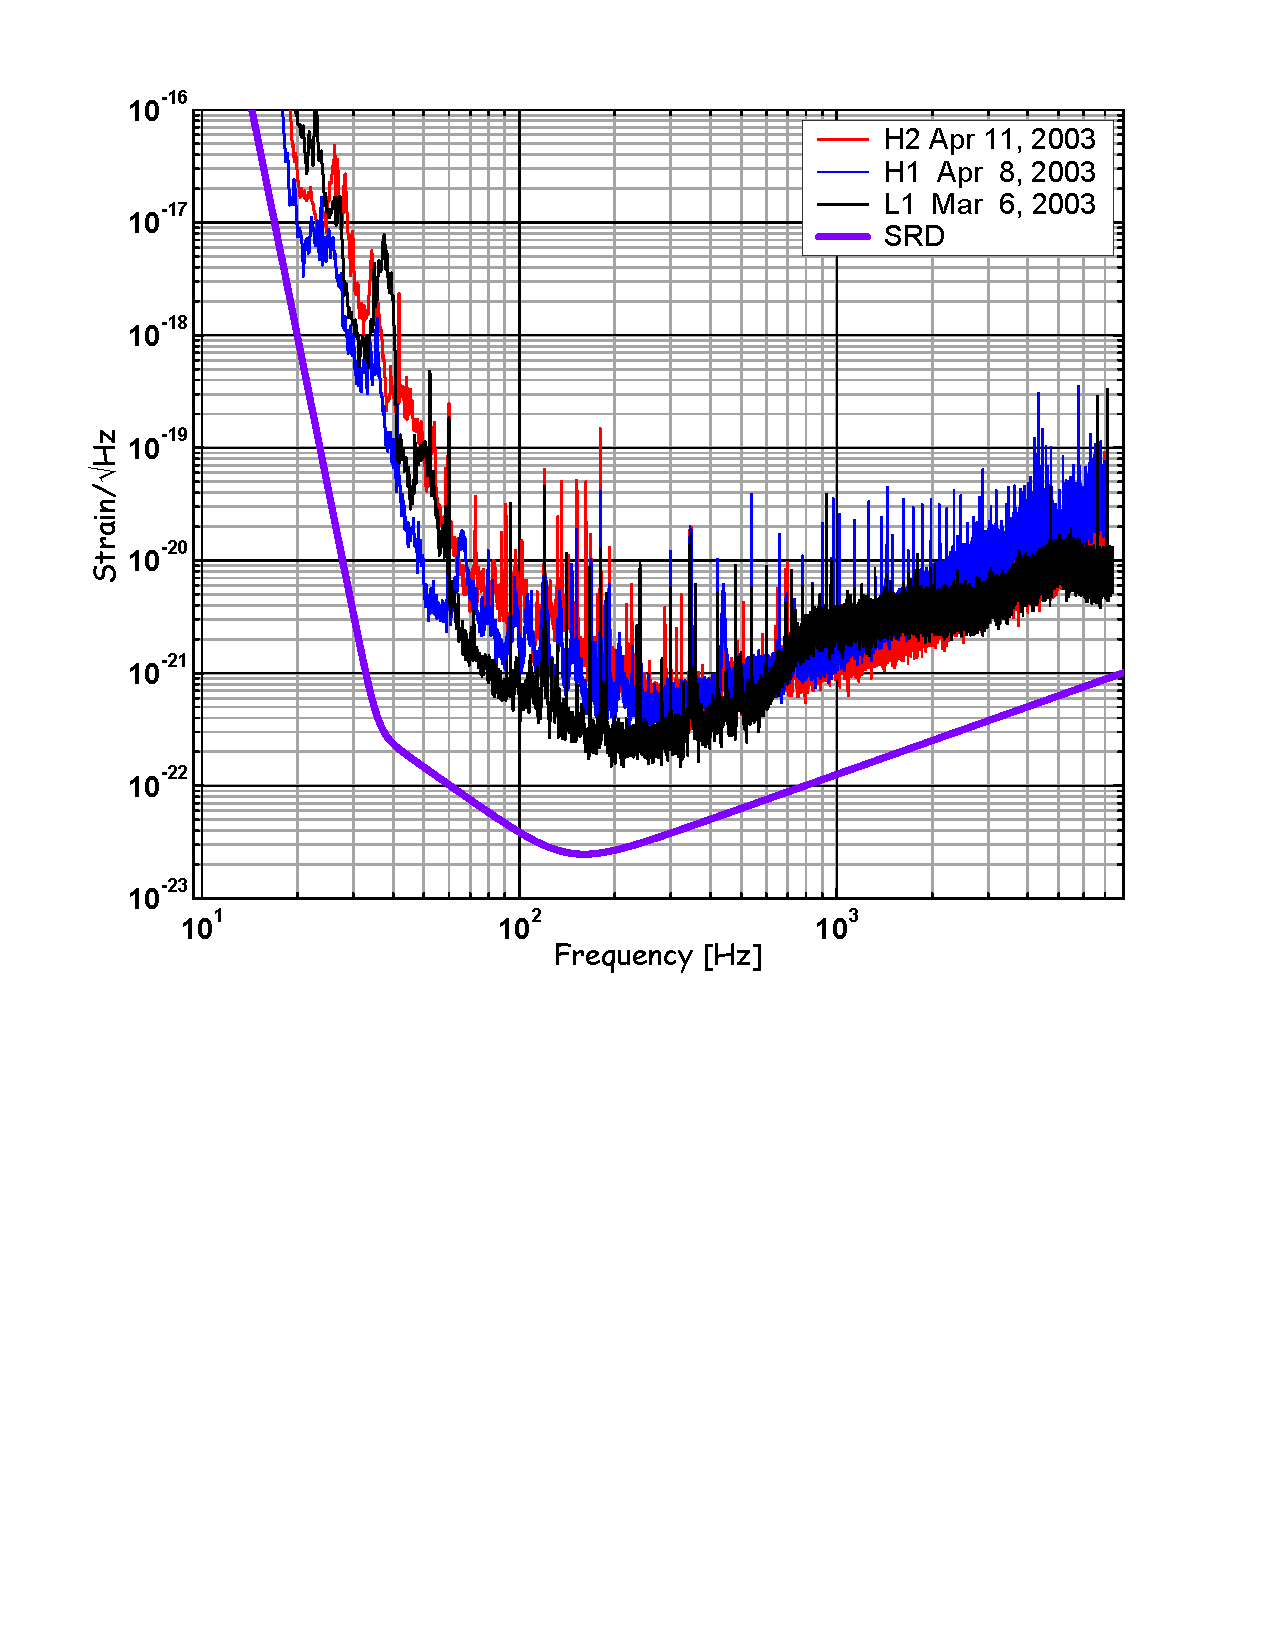
\includegraphics[angle=0,width=6.5in]{Figures/Chap4/S2noiseComp.pdf}}
\caption[S2 Noise Curves]{Comparison of the interferometer noises during the
           second Science Run (S2).}
\label{fig:S2noiseComp}
\end{figure}


\begin{figure}[!h]
\centerline{
\includegraphics[angle=0,width=6.5in]{Figures/Chap4/S3noiseComp.pdf}}
\caption[S3 Noise Curves]{Comparison of the interferometer noises during the
           third Science Run (S3).}
\label{fig:S3noiseComp}
\end{figure}


\subsection{Evolution of Phase Sensitivity}

The original Michelson interferometers were able to resolve
down to 1\% of an optical fringe. The LIGO sensitivity goal requires a phase
noise level of $3.5 \times 10^{-11}$ radians/$\sqrt{\mbox{Hz}}$. This very
small phase shift can be sensed due mainly to the increased power levels
in the Michelson part of the interferometer. Figure~\ref{fig:PhaseNoise}
shows the evolution of optical phase noise measurements in the last 40 years.

\begin{figure}[!h]
\centerline{
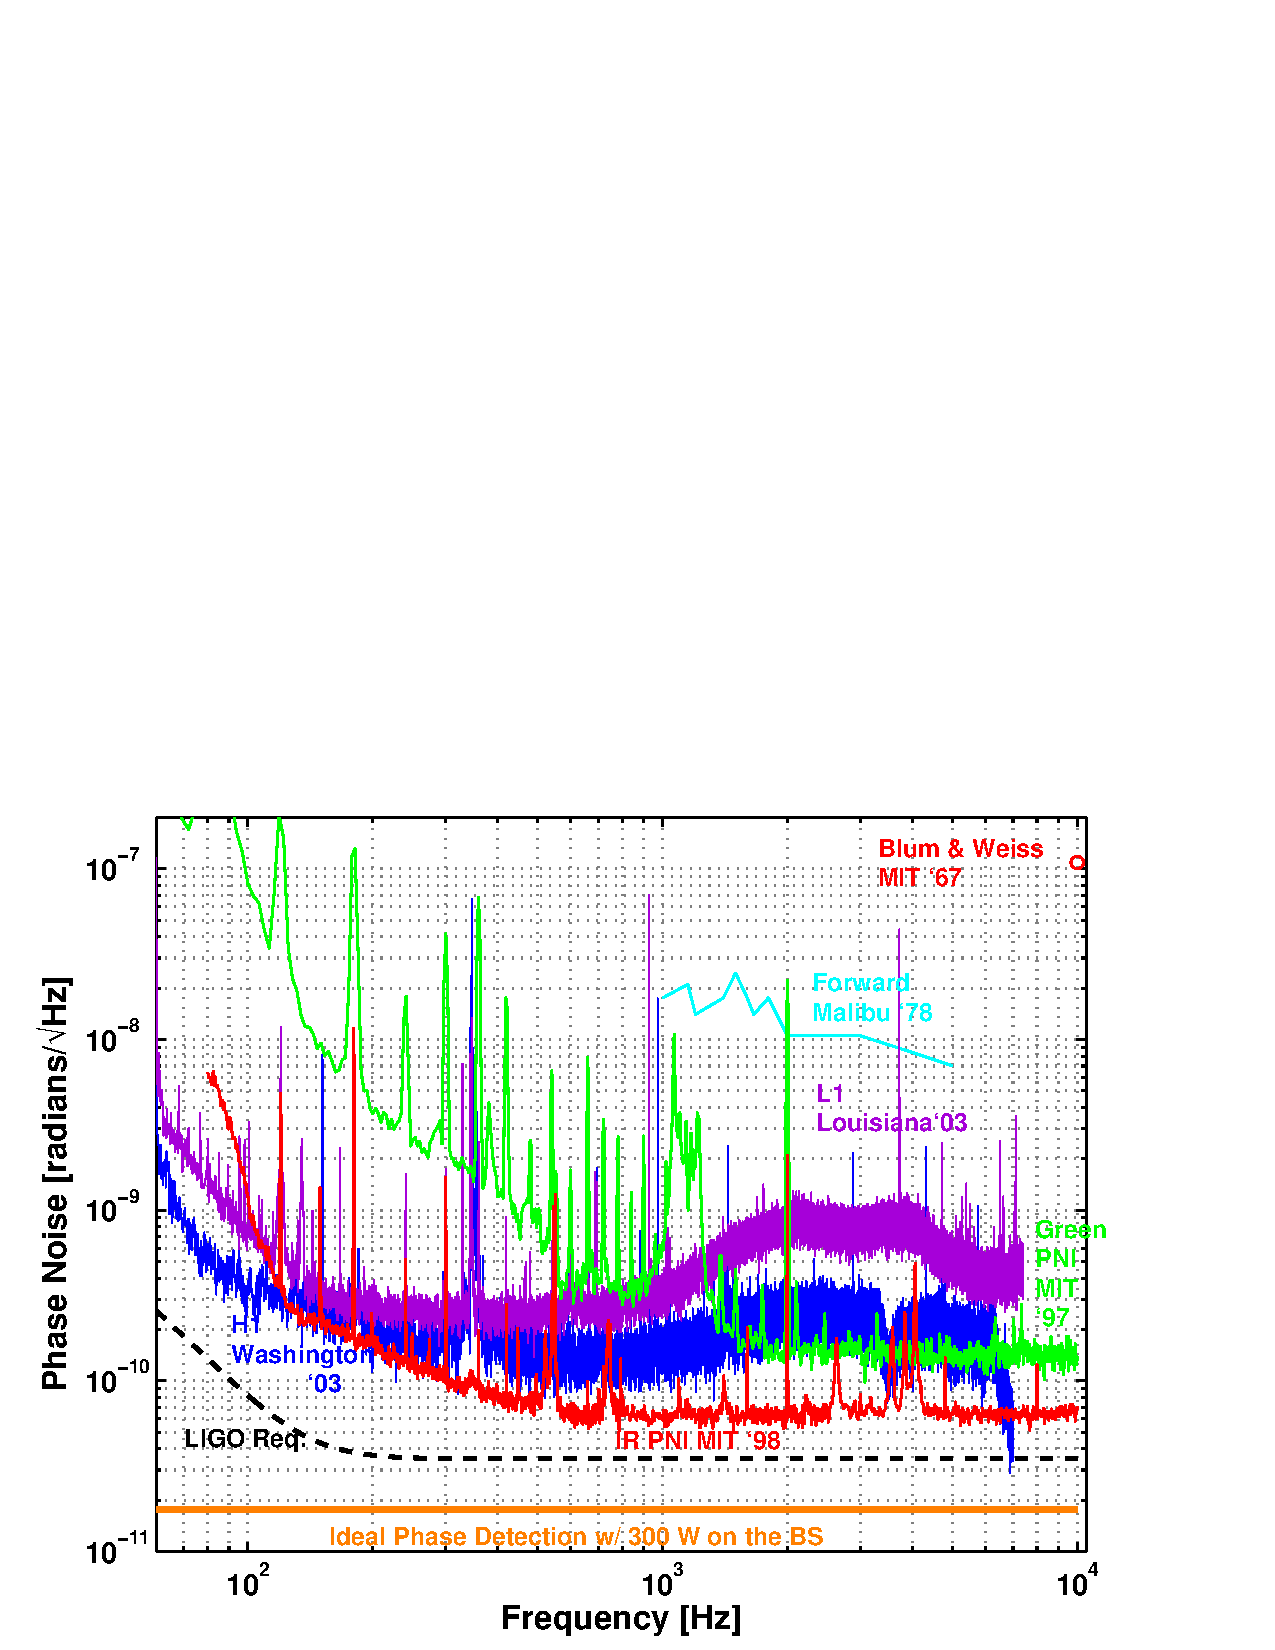
\includegraphics[angle=0,width=6.5in]{Figures/Chap4/PhaseNoises.pdf}}
\caption[Phase Noise]{Evolution of Phase Noise Measurements. The phase shift
         here is defined as the single trip difference between the two arms.
         This convention makes all of the curves a factor of 2 lower than
         in other phase noise comparisons~\cite{Brian:Thesis,Fritschel:PNI}}
\label{fig:PhaseNoise}
\end{figure}


